\chapter{Conceptual Model}\label{chap:conceptual_model}


\section{Introduction}\label{sec:introduction}
Thread mesh wireless networks have gained popularity recently due to their low-power and short-range capabilities, making them ideal for IoT applications. However, optimizing the power consumption in these networks remains a challenge. This chapter presents a conceptual model for overall power optimization in Thread mesh wireless networks by algorithmizing parameters. The following image incorporates a representative network image, illustrating the key components of a Thread mesh network.

\begin{figure}[h]
    \centering
    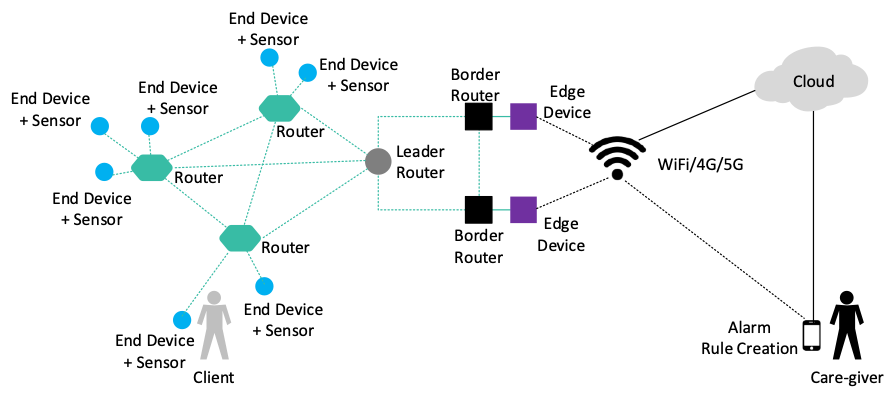
\includegraphics[width=0.8\textwidth]{images/conceptual_model/Thread_mesh_network.png}
    \caption{A representative Thread mesh network.}
    \label{fig:conceptual_model}
\end{figure}


\section{Network Components and Structure}\label{sec:network_components}
The representative network image for a Thread mesh wireless network includes:

\vspace{2mm}
\begin{enumerate}
  \item \textbf{2 Border Routers:} Gateways to external networks, ensuring redundancy and no single point of failure.
  \item \textbf{3 Routers:} Relay messages within the network, with one selected as the leader for managing configurations and operations.
  \item \textbf{(Sleepy) End Devices (SEED):} Low-power devices connected to router parents, conserving energy when not in use, and allowing integration with various devices.
  \item \textbf{2 Edge Devices:} Connected to border routers, serving as bridges or coordinators for external network communication.
  \item \textbf{Wi-Fi or Internet Cloud Service:} Enables interaction with other networks and devices, with mobile devices connected for user control and monitoring.
\end{enumerate}
\vspace{3mm}


\section{Power Optimization Approach}\label{sec:power_optimization_approach}
Several factors contribute to the power consumption in Thread mesh networks, including transmission power, node density, routing algorithms, and network topology. This conceptual model focuses on transmission power optimization, as it plays a significant role in determining the overall power consumption in the network.

\subsection{Monte Carlo Method for Initial Network Nodes Build and Optimization Values}
Monte Carlo Method is a powerful statistical technique for modeling complex systems with random variables. In the Thread mesh wireless networks context, Monte Carlo simulation can generate initial network node builds based on different mathematical constraints with varying node densities, positions, and transmission power levels. These initial builds can then be used as input for the Genetic Algorithm optimization process.

\subsection{Genetic Algorithm for Power Optimization}
The conceptual model integrates Genetic Algorithm, inspired by natural selection, with Monte Carlo simulation to optimize transmission power levels in Thread mesh wireless networks. Monte Carlo simulation generates initial network node builds with varying densities, positions, and power levels, while GA iteratively evaluates, combines, and mutates these builds to find the optimal settings. The fitness function assesses power efficiency and network performance, considering factors like distance and path loss, enabling the model to explore various configurations and converge to a globally optimal solution.

\section{Conclusion}
The proposed conceptual model presents an integrated approach to power optimization in Thread mesh wireless networks, utilizing Genetic Algorithm and Monte Carlo Method to optimize transmission power and initial network node build. By optimizing these critical factors, the model aims to enhance the performance and energy efficiency of the network, ensuring a more sustainable and reliable IoT communication infrastructure.
